\begin{figure}[!hbt]
  \centering
  \subfigure{
    \label{fig:adjust-partition--all}
    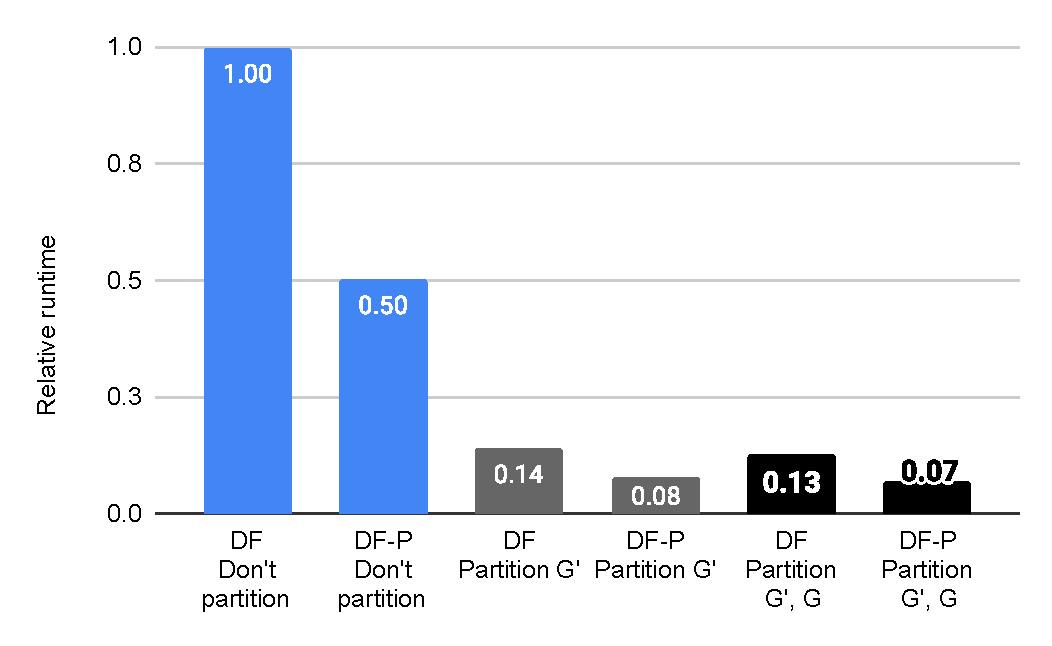
\includegraphics[width=0.98\linewidth]{out/adjust-partition.pdf}
  } \\[-2ex]
  \caption{Mean relative runtime with our \textit{Dynamic Frontier (DF)} and \textit{Dynamic Frontier with Pruning (DF-P)} approaches across three different levels of work-partitioning for GPU computation. Here, \textit{Partition $G$} denotes partitioning the vertices of the current graph $G$ by their out-degree, while \textit{Partition $G^T$} signifies partitioning the vertices by their in-degree.}
  \label{fig:adjust-partition}
\end{figure}
